\chapter{\IfLanguageName{dutch}{Stand van zaken}{State of the art}}%
\label{ch:stand-van-zaken}

% Tip: Begin elk hoofdstuk met een paragraaf inleiding die beschrijft hoe
% dit hoofdstuk past binnen het geheel van de bachelorproef. Geef in het
% bijzonder aan wat de link is met het vorige en volgende hoofdstuk.

% Pas na deze inleidende paragraaf komt de eerste sectiehoofding.

\begin{comment}

Dit hoofdstuk bevat je literatuurstudie. De inhoud gaat verder op de inleiding, maar zal het onderwerp van de bachelorproef *diepgaand* uitspitten. De bedoeling is dat de lezer na lezing van dit hoofdstuk helemaal op de hoogte is van de huidige stand van zaken (state-of-the-art) in het onderzoeksdomein. Iemand die niet vertrouwd is met het onderwerp, weet nu voldoende om de rest van het verhaal te kunnen volgen, zonder dat die er nog andere informatie moet over opzoeken \autocite{Pollefliet2011}.

Je verwijst bij elke bewering die je doet, vakterm die je introduceert, enz.\ naar je bronnen. In \LaTeX{} kan dat met het commando \texttt{$\backslash${textcite\{\}}} of \texttt{$\backslash${autocite\{\}}}. Als argument van het commando geef je de ``sleutel'' van een ``record'' in een bibliografische databank in het Bib\LaTeX{}-formaat (een tekstbestand). Als je expliciet naar de auteur verwijst in de zin, gebruik je \texttt{$\backslash${}textcite\{\}}.
Soms wil je de auteur niet expliciet vernoemen, dan gebruik je \texttt{$\backslash${}autocite\{\}}. In de volgende paragraaf een voorbeeld van elk.

\textcite{Knuth1998} schreef een van de standaardwerken over sorteer- en zoekalgoritmen. Experten zijn het erover eens dat cloud computing een interessante opportuniteit vormen, zowel voor gebruikers als voor dienstverleners op vlak van informatietechnologie~\autocite{Creeger2009}.

\end{comment}

% TODO: SVZ korte introductie meegeven ...


\section{Wat is Microsoft administration?}

% Taalcheck OK

Microsoft administration bestaat uit twee kernwoorden die bekend zijn binnen de \ac{IT}-wereld. Microsoft staat voor het Amerikaanse technologiebedrijf en de producten dat het aanbiedt \autocite{Warner2019}. Het woord administration, oftewel administratie in het Nederlands, staat voor het beheren van iets \autocite{Burgess2003}. Vanuit het woord administration volgde het woord administrator, dat duidt op een persoon die een of meerdere instanties beheert. Kortom, Microsoft administration staat voor het beheren van Microsoft-instanties en -producten (bv. Windows en Azure). 

% TODO: bv. & IT afkorting ergens noteren over zorgen dat dit hierboven komt en dan een “ac” erover maken 

\subsection{Administration in de jaren tachtig en negentig}

% Taalcheck OK

Het beheren van systemen kan omvat worden in enkele taken, hieronder volgt een lijst van frequente taken tussen het jaar 1980 en 2000 \autocite{Frisch2002}.

\begin{itemize}
    \item Toevoegen van nieuwe gebruikers en toestellen
    \item Maken en beheren van back-ups
    \item Bestanden en andere data recupereren
    \item Gebruikers assisteren in dagelijkse taken en problemen
    \item Monitoren van systemen
    \item De veiligheid van de systemen garanderen
    \item Het beheren en installeren van updates
    \item Het automatiseren van taken
\end{itemize}

Deze taken zijn vandaag de dag nog steeds herkenbaar als dagdagelijkse taken van een systeembeheerder. 

\subsection{Microsoft administration via Windows}

% Taalcheck OK

Sinds de opkomst van Windows-systemen zoals Windows 2000 server, zijn er mogelijkheden om administratieve taken uit te voeren binnen netwerkinfrastructuren \autocite{Tulloch2001}. \\

Binnen Windows 2000 server zijn er administratieve tools zoals Microsoft Management Console, Event Viewer en Active Directory Domains and Trusts-instellingen beschikbaar. Deze tools dienen om de taken van een administrator te vergemakkelijken, door een overzicht te brengen van alle data in dat specifieke onderdeel \autocite{Sibisi2022}. Door het gebruik van deze administratieve tools kan een administrator Microsoft-entiteiten waaronder Windows-toestellen beheren om zijn taken mee uit te voeren. 

\subsection{Hoe evolueerde de systemen en de administratie hiervan doorheen de jaren?}

% Taalcheck OK

In het begin van de eenentwintigste eeuw werden systemen en servers zoals Windows 2000 server met een focus op \ac{On-prem} onderhouden \autocite{Microsoft2022a}. \ac{On-prem} betekent dat software en hardware, zoals computers en servers, op locaties staan dat eigendom is van het bedrijf en lokaal worden toegepast \autocite{Gastermann2015}. Hierbij wordt de systeemadministratie door systeembeheerders lokaal aangepakt. Ter illustratie, in dit scenario focust de automatisatie via PowerShell zich op de lokale entiteiten binnen het bedrijf. Databanken, mailservers, \ac{DNS}-servers en andere instanties worden lokaal aangesproken en geautomatiseerd indien nodig. \\

Rond het jaar 2006 evolueerde de On-premises-aanpak naar een cloud-aanpak \autocite{Hayes2008}. EC2 van Amazon is een van de grondleggers binnen de cloudservices \autocite{Qian2009}. Deze inventie van Amazon heeft sindsdien invloed op de huidige marktleiderspositie van AWS in cloud computing \autocite{Vailshery2022}. Op de tweede plaats bevindt zich de cloudservice van Microsoft, genaamd Azure.

\subsection{De impact van cloud computing}

% Taalcheck OK

Cloud computing heeft een brede betekenis. Het is in feite een technologiemodel die wordt gebruikt om middelen en diensten beschikbaar te stellen op het internet, of de cloud. \autocite{Haag2009} \\

De migratie van \ac{On-prem} naar de cloud is geen toeval. Eenenveertig procent van de bedrijven uit de \ac{EU} maakt gebruik van cloud computing in 2021 \autocite{EU2021}. Het gebruik van cloud computing en cloudservices heeft vele voordelen. De volgende lijst bevat enkele voordelen van cloud computing. De lijst is samengesteld uit onderzoek van \textcite{Aljabre2012}, \textcite{Rittinghouse2016}.

\begin{itemize}
    \item Minder onderhouds-, implementatie- en infrastructuurkosten.
    \item Goedkopere computers per gebruiker (via virtuele machines).
    \item Verhoogde mobiliteitskansen voor de werkkrachten.
    \item Nieuwe en flexibelere infrastructuren met verhoogde schaalbaarheid.
    \item Vergroening van data centers.
    \item Verhoogde beschikbaarheid van applicaties.
    \item Mogelijkheid om gebruikers te doen samenwerking in documenten en projecten.
     
\end{itemize}

\subsection{Welke impact heeft de verschuiving van On-premises naar de cloud op Microsoft administration?}

% Taalcheck

De evolutie van \ac{On-prem} naar de cloud heeft invloed op de huidige stand van zaken binnen Microsoft administration. Microsoft administratie staat in voor het beheren van Microsoft-entiteiten. Door een verschuiving van \ac{On-prem} naar cloudomgevingen, wordt de nadruk stilaan gelegd op het beheren van bepaalde entiteiten via cloudtoepassingen. \\

Deze nadruk valt op wanneer de productenlijst van Microsoft Azure wordt geraadpleegd \autocite{Microsoft2023b}. Dit is een lijst die steeds verder wordt uitgebreid met nieuwe technologieën. \\

Een praktisch voorbeeld van een entiteit, of een groep van entiteiten, dat via de cloud kan beheerd worden is Azure Active Directory \autocite{Microsoft2023c}. Azure Active Directory kan gebruikt worden als alternatief voor Active Directory voor bepaalde onderdelen. Active Directory is kortweg een opslagplaats die een focus heeft op On-premises-instanties. Active Directory en Azure Active Directory worden in het volgende onderdeel verder besproken.

% ---
% Volgende onderdeel
% ---

\section{Azure Active Directory}

\ac{AD} is een centrale en gemeenschappelijke opslagplaats voor informatie geïntroduceerd door Microsoft \autocite{Allen2003}. De eerste versie van \ac{AD} is gemaakt voor de Windows 2000 server-editie. Deze opslagplaats bevat allerlei informatie binnen een netwerk, zoals gebruikers, groepen, computers, applicaties, bestanden en printers. Deze informatie kan worden opgevraagd en beheerd. \\

Azure \ac{AD} is een modernere aanpak van Active Directory binnen de cloud dat ontstaan is in 2008 \autocite{Chappell2008}. Azure \ac{AD} is een gecentraliseerd beheerplatform van Microsoft voor gebruikers en apparaten in netwerken die een verbinding hebben met de Azure-clouddienst \autocite{Mayank2019}. Middelen, waaronder gebruikers en apparaten, kunnen vanuit Azure \ac{AD} beheerd worden met bijhorende netwerkauthenticatie. Het dient als een centraal punt van informatie, waarbij details over alle middelen in het netwerk worden opgeslagen.

\subsection{Wat is Azure Active Directory met PowerShell?} 

Azure \ac{AD} PowerShell voor Graph, kortweg Azure \ac{AD} PowerShell, is een module binnen PowerShell dat gebruikt kan worden om Azure \ac{AD} te beheren \autocite{Microsoft2023}. PowerShell is een oplossing van Microsoft voor taakautomatisering via een \ac{CLI} \autocite{Microsoft2022}. \\

PowerShell staat gekend voor zijn breed scala aan informatie dat het kan verkrijgen. Dit breed scala gaat van systemen, servers, randapparatuur, mobiele apparaten tot gegevensgestuurde toepassingen zoals Active Directory \autocite{Hosmer2019}. Vandaag de dag ondersteunt PowerShell meer dan 11.350 unieke modules en scripts via de PowerShell Gallary, waaronder de Azure \ac{AD} PowerShell module \autocite{Microsoft2023a}. \\

Door het gebruik van Azure \ac{AD} in combinatie met PowerShell, wordt er gebruikgemaakt van het beste van de twee werelden. Een gecentraliseerd beheerplatform automatisch doen werken brengt bijkomende voordelen voor de maker. Uit onderzoek van \textcite{Breton2003} zijn enkele voordelen van automatisatie minder stress, tijdbesparing en een lagere kans op menselijke fouten.

\subsection{Wat is Azure Active Directory Graph?}

De communicatie tussen Azure \ac{AD} en de Azure \ac{AD} PowerShell-module gebeurd via een \ac{API}. Deze \ac{API} is een \ac{REST} \ac{API} dat Graph wordt genoemd. \\ 

De naam Graph is afgeleid uit het wiskundige figuur van een graaf. Een graaf is een verzameling van punten die wel of niet met elkaar zijn verbonden \autocite{Denaux2022}. Een voorbeeld van een wiskundige graaf is te zien op Figuur \ref{mga}. \\

\begin{figure}[h]
    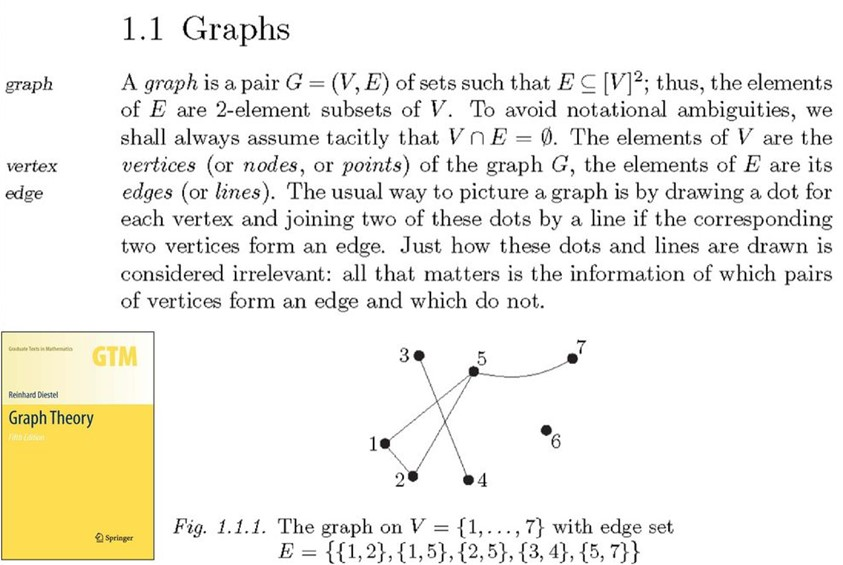
\includegraphics[width=\textwidth]{MathGraphExample.jpg}
    \caption[Voorbeeld wiskundige graaf]{Voorbeeld van een graaf in de wiskunde uit het boek Graph Theory van \textcite{Diestel2010}.}
    \label{mga}
\end{figure}

Graph van Microsoft heeft een soortgelijke betekenis als dat van een wiskundige graaf. Graph staat in voor de verbindingen tussen de entiteiten dat het ondersteunt, in dit geval Microsoft-entiteiten \autocite{Kokkarinen2022}. Een logische interpretatie van Graph wordt weergegeven op Figuur \ref{gms}. \\

\begin{figure}[h]
    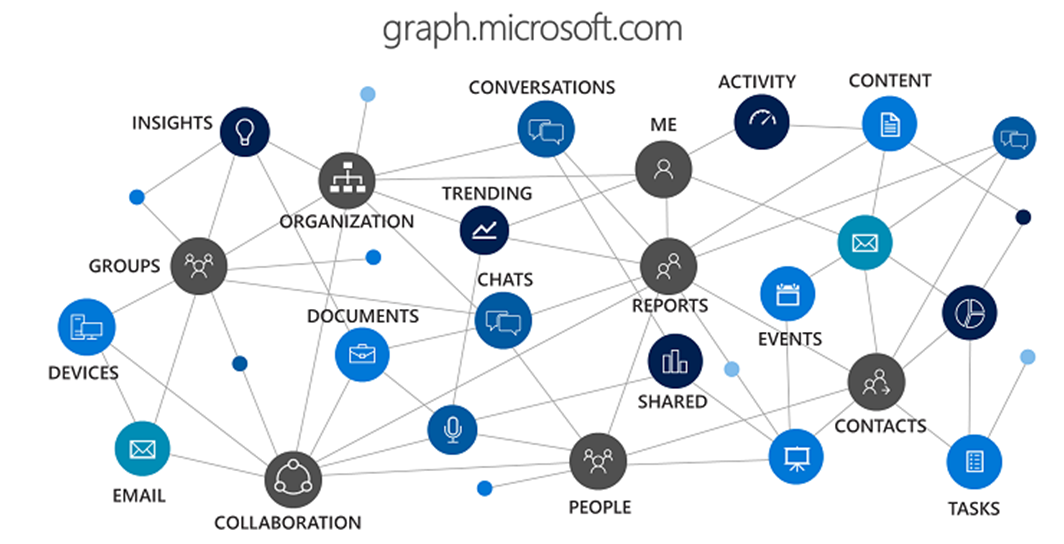
\includegraphics[width=\textwidth]{GraphMicrosoft.png}
    \caption[Voorbeeld Azure \ac{AD} Graph]{Voorstelling van Azure \ac{AD} Graph door \textcite{Microsoft2017}.}
    \label{gms}
\end{figure}

\subsubsection{Achterliggende werking van Azure Active Directory Graph API}

% TODO: Bronnen (zie word onder Azure AD Graph API)

% TODO: Schrijf verder vanuit de bron van weareminky, dit is de makkelijkste manier

De Azure \ac{AD} Graph \ac{API} is een OData 3.0-compatibele dienst om objecten zoals gebruikers, groepen en contactpersonen in een tenant te lezen en te wijzigen \autocite{Microsoft2016}. \\

Het OData-protocol dient voor interacties met gegevens via \ac{REST}-webdiensten. Dit protocol biedt een uniforme manier om gegevens en gegevensmodellen te beschrijven \autocite{OData2023}. \\

Door het gebruik van \ac{REST}-eindpunten kunnen \ac{HTTP}-verzoeken verstuurd worden om bewerkingen uit te voeren met de service. De Azure \ac{AD} Graph \ac{API} heeft een eigen demo-omgeving genaamd Azure \ac{AD} Graph Explorer, waarin bepaalde functies en bewerkingen worden getest \autocite{Microsoft}. \\

Het proces van Graph gaat van start wanneer een applicatie een verzoek doet. Dit verzoek moet een token bevatten. Deze token wordt gegeven door Azure \ac{AD} en bewijst dat de gebruiker de juiste machtigingen heeft om de gevraagde data te raadplegen.

\subsubsection{Authenticatie en autorisatie}

Azure Active Directory-tokens bevatten informatie over de applicatie, de gebruiker, authenticatie en de rechten die een applicatie mag uitvoeren op de bijhorende directory \autocite{Microsoft2015}. \\

Deze tokens bevinden zich in de autorisatieheader van een verzoek.
Een afgekort voorbeeld hiervan is te zien op Figuur \ref{ahtoken}. \\

\begin{figure}[h]
    \begin{verbatim}Authorization: Bearer eyJ0eX ... FWSXfwtQ
    \end{verbatim}    
    \caption[Voorbeeld Azure AD-token]{Afgekort voorbeeld van een Azure AD-token binnen een autorisatieheader.}
    \label{ahtoken}
\end{figure}

Vervolgens voert de \ac{API} de nodige autorisaties uit via permissie scopes. Dit zijn OAuth 2.0 permissie scopes die aanwezig zijn in het Azure \Ac{AD}-token. OAuth 2.0 is een standaardprotocol voor autorisatie \autocite{OAuth}. \\

De permissie scopes worden gebruikt om te controleren of een gebruiker toegang heeft tot een bepaalde map of locatie. Een ontwikkelaar moet in dit scenario de juiste permissie scopes gebruiken om over de vereiste rechten te beschikken voor een actie. \\

Wanneer er wordt aangemeld, krijgt de gebruiker de mogelijkheid om toestemming te geven of de applicatie in kwestie de mapgegevens van de gebruiker mag benutten. Tijdens het toestaan worden de permissie scopes meegegeven die de ontwikkelaar heeft ingesteld. Een opsomming van de mogelijk permissie scopes binnen de Azure \ac{AD} Graph \ac{API} bevindt zich hieronder. 

\begin{itemize}
    \item User.Read: Rechten om aan te melden en het gebruikersprofiel te lezen.
    \item User.Readbasic.All: Rechten om de basisprofielen van alle gebruikers te lezen.
    \item User.Read.All: Rechten om het volledige profiel van alle gebruikers te lezen.
    \item Group.Read.All: Rechten om alle groepen te lezen.
    \item Group.ReadWrite.All: Rechten om alle groepen te lezen en te bewerken
    \item Device.ReadWrite.All: Rechten om alle apparaten te lezen en te bewerken.
    \item Directory.Read.All: Rechten om alle mapgegevens te lezen.
    \item Directory.ReadWrite.All: Rechten om alle mapgegevens te lezen en te bewerken.
    \item Directory.AccessAsUser.All: Rechten om in de map toe treden als de aangemelde gebruiker.
\end{itemize}

Het gebruik van permissie scopes komt overeen met een gekend veiligheidsprincipe binnen de \ac{IT}. “Principle of Least Privilege”, of “Beginsel van de minste voorrechten” in het Nederlands, staat voor het toekennen van een minimum aan rechten \autocite{Saltzer1975}. 

\subsubsection{Eindpunt adressering}

% TODO: foto's zoeken om het makkelijker te maken?

Om taken of functies uit te voeren met de Graph \ac{API}, wordt er gebruikgemaakt van \ac{HTTP}-verzoeken. Deze verzoeken maken gebruik van een bepaalde methode. Een opsomming van de mogelijk methodes wordt hieronder weergegeven met bijhorende betekenis, gebaseerd op het onderzoek van \textcite{Fielding1999}, \textcite{Dusseault2010}.

\begin{itemize}
    \item GET: Geeft data weer van de server.
    \item POST: Verstuurt data naar de server om nieuwe data aan te maken.
    \item PATCH: Verstuurt data naar de server om gedeeltelijk de bron bij te werken.
    \item PUT: Verstuurt data naar de server om de volledige bron bij te werken.
    \item DELETE: Verwijdert data van de server.
\end{itemize}

Deze verzoeken zijn gericht op een eindpunt van een dienst, rescource, een verzameling of rescource of andere entiteiten die de \ac{API} ondersteunt. De eindpunten worden genoteerd als een \ac{URL}. Het gebruikelijk formaat van zo'n eindpunt wordt voorgesteld op Figuur \ref{bfe}. \\

\begin{figure}[h]
    \begin{verbatim}https://graph.windows.net/{tenant_id}/{resource_path}?{api_version}
    \end{verbatim}    
    \caption[Basis formaat Graph API-eindpunt]{Het basis formaat van een Graph API-eindpunt.}
    \label{bfe}
\end{figure}

De reeds voorgestelde \ac{URL} bestaat uit vier componenten.

\begin{itemize}
    \item Service root: Het aanspreekpunt voor alle Graph \ac{API}-verzoeken. Voor Azure \ac{AD} Graph is dit “https://graph.windows.net”.
    \item Tenant Identifier: De identiteit van de tenant waar het verzoek naar gericht is.
    \item Rescource path: Het pad van de bron waar het verzoek naar gericht is.
    \item Graph \ac{API} version: De versie van de \ac{API} waar het verzoek naar gericht is.
\end{itemize}

Een praktisch voorbeeld met betrekking tot het oproepen van gebruikersgegevens, wordt weergegeven op Figuur \ref{pfe}. \\

\begin{figure}[h]
    \begin{verbatim}https://graph.windows.net/contoso.com/users/john@contoso.com/
$links/manager?api-version=1.6
    \end{verbatim}    
    \caption[Voorbeeld Graph \ac{API}-eindpunt]{Praktisch voorbeeld van een Graph \ac{API}-eindpunt, gericht op de manager eigenschap van “john@contoso.com”.}
    \label{pfe}
\end{figure}

\subsubsection{OData Query Parameters}

Zoals reeds vermeld maar de Graph \ac{API} gebruik van OData. Het gebruik van OData-queryparameters zorgt ervoor dat een ingelezen verzameling van bronnen kunnen gefilterd, gesorteerd en gepagineerd worden. \\

De Graph \ac{API} biedt ondersteuning aan voor de volgende parameters met bijhorende betekenis. De betekenissen staan gedefinieerd in studies van \textcite{Liang2016}, \textcite{Wojcieszyn2014}. 

\begin{itemize}
    \item \$batch: Indienen van \ac{HTTP} POST-verzoeken.
    \item \$expand: Opnemen van een of meerdere bronnen in het antwoord.
    \item \$filter: Filteren van beschikbare bronnen.
    \item \$orderby: Opgeven van ordening door de opgevraagde collectie.
    \item \$previous-page: Ophalen van vorige pagina met resultaten.
    \item \$top: Beperken van een teruggezonden opgevraagde verzameling.
    \item \$skiptoken: Overslaan van opgegeven aantal items.
\end{itemize}

Een toegepast voorbeeld van een OData-queryparameter is te vinden in Figuur \ref{odqp}. \\

\begin{figure}[h]
\begin{verbatim}GET https://graph.windows.net/contoso.com/directoryObjects?api-version=
2013-04-05&$filter=isof('Microsoft.WindowsAzure.ActiveDirectory.User')%20
or%20isof('Microsoft.WindowsAzure.ActiveDirectory.Group')%20
or%20isof('Microsoft.WindowsAzure.ActiveDirectory.Contact')
&deltaLink= HTTP /1.1
\end{verbatim}    
\caption[Voorbeeld OData-queryparamter]{Toegepast voorbeeld van een OData-queryparamter op een \ac{HTTP} GET-request.}
\label{odqp}
\end{figure}

\subsubsection{Request en Response Headers}

% TODO: Bron zoeken voor onderstaande uitleg?

De Graph \ac{API} werkt met verzoeken en antwoorden. Een verzoek werkt met een aantal soorten headers en bodies. \\

Drie voorbeelden van voorkomende verzoekheaders zijn de volgende:

\begin{itemize}
    \item Authorization: Uitgegeven Azure \ac{AD}-token.
    \item Content-Type: Mediatype van de inhoud.
    \item Content-Length: Lengte van het verzoek (in bytes).
\end{itemize} 

Daarnaast bestaan er ook een aantal antwoordheaders. Hieronder worden een aantal mogelijke antwoordheaders meegegeven met hun betekenis.

\begin{itemize}
    \item Content-Type: Mediatype van de inhoud.
    \item Location: Antwoord op POST-verzoeken wanneer een nieuwe bron in de directory wordt aangemaakt.
    \item ocp-aad-diagnostics-server-name: Identifier voor de server die een bewerking uitvoert.
    \item ocp-aad-session-key: Sleutel die een sessie met de directorydienst identificeert.
\end{itemize}

Een voorbeeld van antwoordheaders binnen Azure \ac{AD} Graph wordt weergegeven bij Listing \ref{rhaad}. \\

\begin{listing}[h]
\begin{minted}
[
frame=lines,
framesep=2mm,
baselinestretch=1.2,
fontsize=\footnotesize,
linenos
]  
{json}
{
    "cache-control": "no-cache",
    "client-request-id": "140987df-c416-44b8-bf96-16d550256bad",
    "content-length": "12478",
    "content-type": 
        "application/json; 
        odata=minimalmetadata; 
        streaming=true; 
        charset=utf-8",
    "expires": "-1",
    "ocp-aad-session-key": "MzsMU-KCo5fDEUHgzYfj ... hf8ZctaauwL-EZo",
    "pragma": "no-cache",
    "request-id": "c7f02989-6a03-444a-abb2-e3c7993c1ded"
}
    \end{minted}
    \caption[Voorbeeld Response Headers Azure AD Graph]{Voorbeeld van Response Headers binnen Azure \ac{AD} Graph via Azure \Ac{AD} Graph Explorer.}
    \label{rhaad}
\end{listing}

\subsubsection{Request en Response Bodies}

Request bodies kunnen via \Ac{JSON}- of \ac{XML}-payloads verzonden worden voor POST-, PATCH- en PUT-verzoeken. Bovendien kunnen antwoorden (van een server) worden teruggestuurd via \ac{JSON} of \ac{XML}. \\

Het woord “payload” staat voor data die via een pakket of transmissie worden gedragen \autocite{Comer2006}. \\

Deze payloads kunnen in de request bodies gespecifieerd worden via de Content-Type verzoekheader en in antwoorden van Accept-verzoekheaders. \\

Een voorbeeld van een request, met bijhorende request en response body wordt voorgesteld bij Listing \ref{hpr}, \ref{hreqb} en \ref{hresb}. \\

\begin{listing}[h]
\begin{verbatim}
POST https://graph.windows.net/myorganization/users?api-version
\end{verbatim}
\caption[Voorbeeld \Ac{HTTP} POST-resuest]{Voorbeeld van een \ac{HTTP} POST-request binnen Azure \ac{AD} Graph.}
\label{hpr}
\end{listing}

\begin{listing}[!b]
\begin{minted}
[
frame=lines,
framesep=2mm,
baselinestretch=1.2,
fontsize=\footnotesize,
linenos
]  
{json}
{
    "accountEnabled": true,
    "displayName": "Alex Wu",
    "mailNickname": "AlexW",
    "passwordProfile": {
        "password": "Test1234",
        "forceChangePasswordNextLogin": false
    },
    "userPrincipalName": "Alex@a830edad9050849NDA1.onmicrosoft.com"
}
\end{minted}
\caption[Voorbeeld Request Body Azure AD Graph]{Voorbeeld van een Request Body binnen Azure \ac{AD} Graph.}
\label{hreqb}
\end{listing}

\begin{listing}[!t]
\begin{minted}
[
frame=lines,
framesep=2mm,
baselinestretch=1.2,
fontsize=\footnotesize,
linenos
]  
{json}
{
    "odata.metadata": "https://graph.windows.net/myorganization\n
    /$metadata#directoryObjects/Microsoft.DirectoryServices.User/@Element",
    "odata.type": "Microsoft.DirectoryServices.User",
    "objectType": "User",
    "objectId": "84fba1e8-b942-47c9-a10e-a4bee353ce60",
    "deletionTimestamp": null,
    "accountEnabled": true,
    "assignedLicenses": [],
    "assignedPlans": [],
    "city": null,
    "country": null,
    "department": null,
    "dirSyncEnabled": null,
    "displayName": "Alex Wu",
    "facsimileTelephoneNumber": null,
    "givenName": null,
    "immutableId": null,
    "jobTitle": null,
    "lastDirSyncTime": null,
    "mail": null,
    "mailNickname": "AlexW",
    "mobile": null,
    "onPremisesSecurityIdentifier": null,
    "otherMails": [],
    "passwordPolicies": null,
    "passwordProfile": null,
    "physicalDeliveryOfficeName": null,
    "postalCode": null,
    "preferredLanguage": null,
    "provisionedPlans": [],
    "provisioningErrors": [],
    "proxyAddresses": [],
    "sipProxyAddress": null,
    "state": null,
    "streetAddress": null,
    "surname": null,
    "telephoneNumber": null,
    "usageLocation": null,
    "userPrincipalName": "alex@a830edad9050849NDA1.com",
    "userType": "Member"
}
\end{minted}
\caption[Voorbeeld Response Body Azure AD Graph]{Voorbeeld van een Response Body binnen Azure \ac{AD} Graph.}
\label{hresb}
\end{listing}

\subsection{Toepassingen van Azure AD via PowerShell en Graph} 

% TODO... (Reserve)

Idee: reeds recente voorbeelden illustreren...

Vb. Applicatie voor Teams via de Graph API... 

% ---
% Volgend onderdeel
% ---

\section{Microsoft Graph}

Microsoft Graph is, net zoals de reeds besproken Azure \Ac{AD} Graph, een centrale \ac{REST} \ac{API} voor Microsoft-entiteiten. Deze technologie werd door \textcite{Microsoft2015a} in de schijnwerper gezet in 2015. \\

De technologie is gebasseerd op de wiskundige graaf, zoals ook reeds besproken werd bij Azure \Ac{AD} Graph. Microsoft Graph integreert applicaties met verschillende programmeertalen en platformen. Het logisch concept van Graph wordt weergegeven op Figuur \ref{msg}.

\begin{figure}[h]
    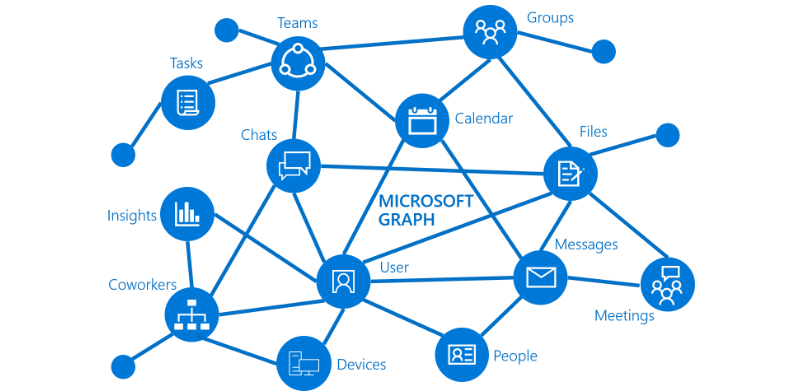
\includegraphics[width=\textwidth]{MicrosoftGraph.png}
    \caption[Voorbeeld Microsoft Graph]{Voorstelling van Microsoft Graph door \textcite{Microsoft2023d}.}
    \label{msg}
\end{figure}

\subsection{Waarom Microsoft Graph als vervanger?} 
Microsoft Graph is de opvolger van de Azure \ac{AD} PowerShell-modules en bijhorende Azure \Ac{AD} Graph. Op 30 september 2022 maakte Microsoft (BRON uitfasering???) bekend dat de uitfasering van de Azure \ac{AD} PowerShell-modules van start zou gaan op 30 juni 2023. \\

De reden waarom Microsoft deze overgang in gang zet, ontstaat uit volgende redenen volgens \textcite{Microsoft2023e}:

\begin{itemize}
    \item Het gebruik van Microsoft Graph ligt dubbel zo hoog dan dat van Azure \ac{AD} Graph.
    \item Microsoft Graph bevat meer dan 150 nieuwe functies.
    \item Microsoft Graph biedt meer veiligheid en is veerkrachtiger.
    \item Microsoft Graph client libraries bevatten een ingebouwde ondersteuning voor bepaalde functies, waaronder
    \begin{itemize}
        \item herhaalde verwerkingshandelingen,
        \item veilige doorverwijzing,
        \item transparante verificatie,
        \item en payloadcompressie.
    \end{itemize}
    \item Verbeterde mogelijkheden zoals Microsoft 365-groepsbeheer, uitnodiging voor externe gebruikers en anderen.
\end{itemize} 

% TODO Verder schrijven? Navragen!!!

\subsection{Achterliggende werking van Microsoft Graph}

% TODO: \subsubsection{MSAL ...}



\subsection{Toepassingen van Microsoft Graph}